%-----------------------------------------------------------------------------------------------------------------------------------------------%
%	The MIT License (MIT)
%
%	Copyright (c) 2019 Jan Küster
%
%	Permission is hereby granted, free of charge, to any person obtaining a copy
%	of this software and associated documentation files (the "Software"), to deal
%	in the Software without restriction, including without limitation the rights
%	to use, copy, modify, merge, publish, distribute, sublicense, and/or sell
%	copies of the Software, and to permit persons to whom the Software is
%	furnished to do so, subject to the following conditions:
%	
%	THE SOFTWARE IS PROVIDED "AS IS", WITHOUT WARRANTY OF ANY KIND, EXPRESS OR
%	IMPLIED, INCLUDING BUT NOT LIMITED TO THE WARRANTIES OF MERCHANTABILITY,
%	FITNESS FOR A PARTICULAR PURPOSE AND NONINFRINGEMENT. IN NO EVENT SHALL THE
%	AUTHORS OR COPYRIGHT HOLDERS BE LIABLE FOR ANY CLAIM, DAMAGES OR OTHER
%	LIABILITY, WHETHER IN AN ACTION OF CONTRACT, TORT OR OTHERWISE, ARISING FROM,
%	OUT OF OR IN CONNECTION WITH THE SOFTWARE OR THE USE OR OTHER DEALINGS IN
%	THE SOFTWARE.
%	
%
%-----------------------------------------------------------------------------------------------------------------------------------------------%


%============================================================================%
%
%	DOCUMENT DEFINITION
%
%============================================================================%

%we use article class because we want to fully customize the page and don't use a cv template
\documentclass[10pt,A4]{ctexart}	


%----------------------------------------------------------------------------------------
%	ENCODING
%----------------------------------------------------------------------------------------

% we use utf8 since we want to build from any machine
\usepackage[utf8]{inputenc}		

%----------------------------------------------------------------------------------------
%	LOGIC
%----------------------------------------------------------------------------------------

% provides \isempty test
\usepackage{xstring, xifthen}

%----------------------------------------------------------------------------------------
%	FONT BASICS
%----------------------------------------------------------------------------------------

% some tex-live fonts - choose your own

%\usepackage[defaultsans]{droidsans}
%\usepackage[default]{comfortaa}
%\usepackage{cmbright}
\usepackage[default]{raleway}
%\usepackage{fetamont}
%\usepackage[default]{gillius}
%\usepackage[light,math]{iwona}
%\usepackage[thin]{roboto} 

% set font default
\renewcommand*\familydefault{\sfdefault} 	
\usepackage[T1]{fontenc}

% more font size definitions
\usepackage{moresize}

%----------------------------------------------------------------------------------------
%	FONT AWESOME ICONS
%---------------------------------------------------------------------------------------- 

% include the fontawesome icon set
\usepackage{fontawesome}

% use to vertically center content
% credits to: http://tex.stackexchange.com/questions/7219/how-to-vertically-center-two-images-next-to-each-other
\newcommand{\vcenteredinclude}[1]{\begingroup
\setbox0=\hbox{\includegraphics{#1}}%
\parbox{\wd0}{\box0}\endgroup}

% use to vertically center content
% credits to: http://tex.stackexchange.com/questions/7219/how-to-vertically-center-two-images-next-to-each-other
\newcommand*{\vcenteredhbox}[1]{\begingroup
\setbox0=\hbox{#1}\parbox{\wd0}{\box0}\endgroup}

% icon shortcut
\newcommand{\icon}[3] { 							
	\makebox(#2, #2){\textcolor{maincol}{\csname fa#1\endcsname}}
}	

% icon with text shortcut
\newcommand{\icontext}[4]{ 						
	\vcenteredhbox{\icon{#1}{#2}{#3}}  \hspace{2pt}  \parbox{0.9\mpwidth}{\textcolor{#4}{#3}}
}

% icon with website url
\newcommand{\iconhref}[5]{ 						
    \vcenteredhbox{\icon{#1}{#2}{#5}}  \hspace{2pt} \href{#4}{\textcolor{#5}{#3}}
}

% icon with email link
\newcommand{\iconemail}[5]{ 						
    \vcenteredhbox{\icon{#1}{#2}{#5}}  \hspace{2pt} \href{mailto:#4}{\textcolor{#5}{#3}}
}

%----------------------------------------------------------------------------------------
%	PAGE LAYOUT  DEFINITIONS
%----------------------------------------------------------------------------------------

% page outer frames (debug-only)
% \usepackage{showframe}		

% we use paracol to display breakable two columns
\usepackage{paracol}

% define page styles using geometry
\usepackage[a4paper]{geometry}

% remove all possible margins
\geometry{top=1cm, bottom=1cm, left=1cm, right=1cm}

\usepackage{fancyhdr}
\pagestyle{empty}

% space between header and content
% \setlength{\headheight}{0pt}

% indentation is zero
\setlength{\parindent}{0mm}

%----------------------------------------------------------------------------------------
%	TABLE /ARRAY DEFINITIONS
%---------------------------------------------------------------------------------------- 

% extended aligning of tabular cells
\usepackage{array}

% custom column right-align with fixed width
% use like p{size} but via x{size}
\newcolumntype{x}[1]{%
>{\raggedleft\hspace{0pt}}p{#1}}%


%----------------------------------------------------------------------------------------
%	GRAPHICS DEFINITIONS
%---------------------------------------------------------------------------------------- 

%for header image
\usepackage{graphicx}

% use this for floating figures
% \usepackage{wrapfig}
% \usepackage{float}
% \floatstyle{boxed} 
% \restylefloat{figure}

%for drawing graphics		
\usepackage{tikz}				
\usetikzlibrary{shapes, backgrounds,mindmap, trees}

%----------------------------------------------------------------------------------------
%	Color DEFINITIONS
%---------------------------------------------------------------------------------------- 
\usepackage{transparent}
\usepackage{color}

% primary color
\definecolor{maincol}{RGB}{ 225, 0, 0 }

% accent color, secondary
% \definecolor{accentcol}{RGB}{ 250, 150, 10 }

% dark color
\definecolor{darkcol}{RGB}{ 70, 70, 70 }

% light color
\definecolor{lightcol}{RGB}{245,245,245}


% Package for links, must be the last package used
\usepackage[hidelinks]{hyperref}

% returns minipage width minus two times \fboxsep
% to keep padding included in width calculations
% can also be used for other boxes / environments
\newcommand{\mpwidth}{\linewidth-\fboxsep-\fboxsep}
	


%============================================================================%
%
%	CV COMMANDS
%
%============================================================================%

%----------------------------------------------------------------------------------------
%	 CV LIST
%----------------------------------------------------------------------------------------

% renders a standard latex list but abstracts away the environment definition (begin/end)
\newcommand{\cvlist}[1] {
	\begin{itemize}{#1}\end{itemize}
}

%----------------------------------------------------------------------------------------
%	 CV TEXT
%----------------------------------------------------------------------------------------

% base class to wrap any text based stuff here. Renders like a paragraph.
% Allows complex commands to be passed, too.
% param 1: *any
\newcommand{\cvtext}[1] {
	\begin{tabular*}{1\mpwidth}{p{0.98\mpwidth}}
		\parbox{1\mpwidth}{#1}
	\end{tabular*}
}

%----------------------------------------------------------------------------------------
%	CV SECTION
%----------------------------------------------------------------------------------------

% Renders a a CV section headline with a nice underline in main color.
% param 1: section title
\newcommand{\cvsection}[1] {
	\vspace{14pt}
	\cvtext{
		\textbf{\LARGE{\textcolor{darkcol}{\uppercase{#1}}}}\\[-4pt]
		\textcolor{maincol}{ \rule{0.1\textwidth}{2pt} } \\
	}
}

%----------------------------------------------------------------------------------------
%	META SKILL
%----------------------------------------------------------------------------------------

% Renders a progress-bar to indicate a certain skill in percent.
% param 1: name of the skill / tech / etc.
% param 2: level (for example in years)
% param 3: percent, values range from 0 to 1
\newcommand{\cvskill}[3] {
	\begin{tabular*}{1\mpwidth}{p{0.72\mpwidth}  r}
 		\textcolor{black}{\textbf{#1}} & \textcolor{maincol}{#2}\\
	\end{tabular*}%
	
	\hspace{4pt}
	\begin{tikzpicture}[scale=1,rounded corners=2pt,very thin]
		\fill [lightcol] (0,0) rectangle (1\mpwidth, 0.15);
		\fill [maincol] (0,0) rectangle (#3\mpwidth, 0.15);
  	\end{tikzpicture}%
}


%----------------------------------------------------------------------------------------
%	 CV EVENT
%----------------------------------------------------------------------------------------

% Renders a table and a paragraph (cvtext) wrapped in a parbox (to ensure minimum content
% is glued together when a pagebreak appears).
% Additional Information can be passed in text or list form (or other environments).
% the work you did
% param 1: time-frame i.e. Sep 14 - Jan 15 etc.
% param 2:	 event name (job position etc.)
% param 3: Customer, Employer, Industry
% param 4: Short description
% param 5: work done (optional)
% param 6: technologies include (optional)
% param 7: achievements (optional)
\newcommand{\cvevent}[7] {
	
	% we wrap this part in a parbox, so title and description are not separated on a pagebreak
	% if you need more control on page breaks, remove the parbox
	\parbox{\mpwidth}{
		\begin{tabular*}{1\mpwidth}{p{0.72\mpwidth}  r}
	 		\textcolor{black}{\textbf{#2}} & \colorbox{maincol}{\makebox[0.25\mpwidth]{\textcolor{white}{#1}}} \\
			\textcolor{maincol}{\textbf{#3}} & \\
		\end{tabular*}\\[8pt]
	
		\ifthenelse{\isempty{#4}}{}{
			\cvtext{#4}\\
		}
	}

	\ifthenelse{\isempty{#5}}{}{
		\vspace{9pt}
		{#5}
	}

	\ifthenelse{\isempty{#6}}{}{
		\vspace{9pt}
		\cvtext{\textbf{Technologies include:}}\\
		{#6}
	}

	\ifthenelse{\isempty{#7}}{}{
		\vspace{9pt}
		\cvtext{\textbf{Achievements include:}}\\
		{#7}
	}
	\vspace{14pt}
}

%----------------------------------------------------------------------------------------
%	 CV META EVENT
%----------------------------------------------------------------------------------------

% Renders a CV event on the sidebar
% param 1: title
% param 2: subtitle (optional)
% param 3: customer, employer, etc,. (optional)
% param 4: info text (optional)
\newcommand{\cvmetaevent}[4] {
	\textcolor{maincol} {\cvtext{\textbf{\begin{flushleft}#1\end{flushleft}}}}

	\ifthenelse{\isempty{#2}}{}{
	\textcolor{darkcol} {\cvtext{\textbf{#2}} }
	}

	\ifthenelse{\isempty{#3}}{}{
		\cvtext{{ \textcolor{darkcol} {#3} }}\\
	}

	\cvtext{#4}\\[14pt]
}

%---------------------------------------------------------------------------------------
%	QR CODE
%----------------------------------------------------------------------------------------

% Renders a qrcode image (centered, relative to the parentwidth)
% param 1: percent width, from 0 to 1
\newcommand{\cvqrcode}[1] {
	\begin{center}
		
\includegraphics[width={#1}\mpwidth]{qdq}
	\end{center}
}


%============================================================================%
%
%
%
%	DOCUMENT CONTENT
%
%
%
%============================================================================%
\begin{document}
\columnratio{0.31}
\setlength{\columnsep}{2.2em}
\setlength{\columnseprule}{4pt}
\colseprulecolor{lightcol}
\begin{paracol}{2}
\begin{leftcolumn}
%---------------------------------------------------------------------------------------
%	META IMAGE
%----------------------------------------------------------------------------------------
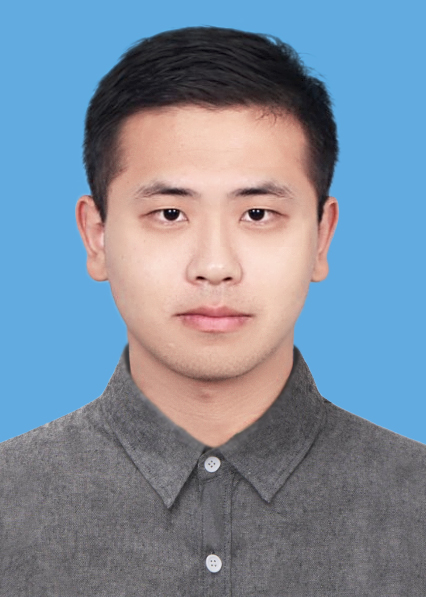
\includegraphics[width=\linewidth]{zpf.jpg}	%trimming relative to image size

%---------------------------------------------------------------------------------------
%	META SKILLS
%----------------------------------------------------------------------------------------
\cvsection{SKILLS}

\cvskill{Python} {5+ yrs} {1} \\[-2pt]

\cvskill{c/c++} {5+ yrs} {1} \\[-2pt]

\cvskill{Rust} {2+ yrs} {0.8} \\[-2pt]

\cvskill{Haskell} {2+ yrs} {0.8} \\[-2pt]

\cvskill{Linux} {5+ yrs} {1} \\[-2pt]

\cvskill{shell} {5+ yrs} {1} \\[-2pt]

\cvskill{Open Source Tools} {5+ yrs} {1} \\[-2pt]

\cvskill{GIT} {3+ yrs} {1} \\[-2pt]

\cvskill{CMAKE} {3+ yrs} {1} \\[-2pt]



\vfill\null
\cvsection{CONTACT}
	
\icontext{MapMarker}{12}{安徽-合肥}{black}\\[6pt]
\icontext{MobilePhone}{12}{130 2322 7925}{black}\\[6pt]
\iconemail{Envelope}{12}{2690955288@qq.com}{2690955288@qq.com}{black}\\[6pt]

\vfill\null
\cvqrcode{0.7}

%---------------------------------------------------------------------------------------
%	EDUCATION
%----------------------------------------------------------------------------------------
%\newpage
%\cvsection{EDUCATIONS}
%
%\cvmetaevent
%{2009 - 2011}
%{M. Sc. Physics.}
%{Universität Bonn}
%{Main thematic priority of those master studies was numerical time series analysis of non-linear dynamical systems. Besides data analysis and transformation, great importance was attached to fast algorithms and efficient software architecture.
%
%In the master thesis a numerical approach for the detection of the direction of interaction was proposed. Analysis of this new approach was performed with the help computer simulations to find out its limits and to compare it to another commonly used approaches.
%
%This numerical approach was highly optimised for cluster computing and implemented in c++ . For those purposes a distributed computing cluster had to be set up and administrated.}
%
%\cvmetaevent
%{2006 - 2009}
%{B. Sc. Physics.}
%{Universität Bonn}
%{The topic for the bachelor's thesis was 'Feshbach resonance'. A numerical application was built to calculate the diagrams.}
%
%\vfill\null
%\cvqrcode{0.7}

%---------------------------------------------------------------------------------------
%	CERTIFICATION
%----------------------------------------------------------------------------------------
%\newpage
%\cvsection{CERTIFICATIONS}
%
%\cvmetaevent
%{LPIC 1 - Linux administrator}
%{}
%{}
%{Certificate issued by the Linux Professional Institute to prove abilities in Linux administration}
%
%\cvmetaevent
%{IBM InfoSphere Advanced DataStage Essentials}
%{}
%{}
%{Intense course about the ETL technologies and the use of IBM DataStage.}
%
%\cvmetaevent
%{Jump Start Program}
%{}
%{}
%{Two months full-time training in object oriented programming in Java SE/EE, software development, testing and modern enterprise web-frameworks. Other topics were object oriented design patterns, test-driven development, SQL-databases and webservers in Java environment (Tomcat / Glasfish / JBoss / Jety)}
%
%
%\cvmetaevent
%{Online Classes}
%{}
%{}
%{It is important for me to stay up to date with the newest topics in the field of IT. In DevOps it is also important to have a general overview and a hands-on experience on them. Therefore, besides intense article studies, I also keep myself up to date with online classes.}
%
%\vfill
%\cvqrcode{0.7}

\newpage
\mbox{} % hotfix to place qrcode on the bottom when there are not other elements
\vfill
\cvqrcode{0.7}

\end{leftcolumn}
\begin{rightcolumn}
%---------------------------------------------------------------------------------------
%	TITLE  HEADER
%----------------------------------------------------------------------------------------
\fcolorbox{white}{darkcol}{\begin{minipage}[c][3.5cm][c]{1\mpwidth}
	\begin {center}
		\HUGE{ \textbf{ \textcolor{white}{ \uppercase{赵鹏飞} } } } \\[-24pt]
		\textcolor{white}{ \rule{0.1\textwidth}{1.25pt} } \\[4pt]
		\large{ \textcolor{white} {软件开发工程师} }
	\end {center}
\end{minipage}} \\[14pt]
\vspace{-12pt}

%---------------------------------------------------------------------------------------
%	PROFILE
%----------------------------------------------------------------------------------------
\vfill\null
\cvsection{EDUCATION}

\cvmetaevent
{2018 - 2021}
{硕士--理论数学}
{上海交通大学}
{
分析学、基础代数学、代数组合、图论
}

\cvmetaevent
{2013 - 2017}
{学士--理论数学}
{南昌大学}
{
分析学、基础代数学、代数组合、图论

概率论、数理统计、近世代数
}

%\cvtext{IT Consultant with strong theoretical skills and a passion for OpenSource sofware.\\
%
%DevOps Engineer, specialized both in automation and in custom application development, experienced with large projects and heterogeneous infrastructures. The link between development and operations, comfortable in both.\\
%
%Customer-oriented and structured method of working, focused on quality and maintainability. Highly motivated to work in a team, both comfortable in big companies as in small teams.\\
%
%}

%---------------------------------------------------------------------------------------
%	WORK EXPERIENCE
%----------------------------------------------------------------------------------------
\vfill\null
\cvsection{WORK EXPERIENCE}

\cvevent
	{2024.08 - 2025.05}
    {超算智芯(合肥)科技有限公司}
	{算法工程师}
	{本项目聚焦于全同态加密算法的实现与性能优化,并将其应用于大规模模型的推理过程,以提升数据隐私保护能力。}
	{\cvlist{
		\item 开发并实现了支持同态加密的底层基本运算模块,包括加法、减法、乘法及整数除法。
		\item 实现了Programmable Bootstrap功能,从而支持同态加密中的任意复杂运算,增强了系统的灵活性和功能性。
		\item 构建大模型所需的底层运算支持体系,涵盖线性代数运算、激活函数及梯度计算等关键模块。
		\item 设计并实现了高效的全同态加密算法并行化方案,通过利用多线程/分布式计算资源,提高了运算效率达30x。
	}}
	{\cvlist {
		\item c++构建核心算法
		\item 利用CMake构建系统优化项目组织,实现了灵活的编译配置,包括但不限于调试、测试和性能优化版本,有效缩短了开发周期并提高了产品质量。
	}}
	{\cvlist{
		\item 独立完成全同态加密算法的设计与实现,构建了功能完整的原型系统,验证了算法的正确性与可行性。
	}}

\vfill\null
\cvevent
	{2022.07 - 2024.04}
	{外企德科-杭州华为研究所}
	{软件开发工程师-预研与开发}
	{
        2022.09-2024.04 \textbf{gem5 工程支撑}:负责并行模块和 CHI 协议的开发和维护。 梳理相关代码和文档,解决用户提出的相关并行与CHI协议bug,深入研究 了锁的实现和使用,并针对各种bug制定了相应的解决方案。提高了系统稳 定性和团队工作效率,使得 gem5 在不损失精度的情况下提高了 50\% 的效率。 \\
\\
    2023.01-2024.02 \textbf{大容量 LLC 动态 QoS 软硬协同}:负责和华为云的 QoS 合作项目,提升硬件利用效率和云服务性能。完成从需求调研、方 案输出和项目测试。和华为云团队保持紧密合作,高效协调资源分配。成 功完成项目,为云场景性能提升提供了有效解决方案同时输出算法专利 一篇,专利名称《一种黑盒负载性能及需求感知的 LLC QOS 优化方 法》。具备了一定机器学习方向的技术积累,能够熟练使用pytorch推理框架, 能够利用Docker进行算法迁移,掌握perf以及flamegrahp等性能调优工具。\\
    \\
    2022.07-2022.12 \textbf{MRAM 大容量 LLC 可行性和性能受益评估}:负责评 估LLC 使用 MRAM 之后写时延、读时延、LLC 容量对于通用计算场景性 能的影响,写寿命是否满足应用需求的仿真评估。分析梳理相关代码,确定 对应需要修改的参数。确定测试方案,分析选择通用场景具有代表性的用例。 完成10+ 用例测试,输出测试报告1篇。 \\
    }
	{\cvlist{
		\item 熟悉linux 内核原理,熟练运用 linux 进程间通信、多线程编程和线程同步, 了解linux 主流发行版
		\item 了解各种机器学习模型,对卷积神经网络、循环神经网络、transformer原理 有一定理解
		\item 熟练掌握c++现代特性和Boost库以及网络编程
		\item 使用Python 语言快速开发、迭代算法
	}}
	{\cvlist {
		\item 算法开发、系统建模及自动化测试脚本开发
		\item shell/Linux 测试环境搭建以及自动化测试脚本开发
		\item 大模型训练
		\item JupyterNotebook/pandas/Matplotlib 数据分析及可视化处理
	}}
	{\cvlist{
		\item gem5并行模块和 CHI 协议的开发和维护
        \item 大容量 LLC 动态 QoS 软硬协同
	}}

\vfill\null
\cvevent
	{2021.05 - 2022.06}
	{上海星恒保险代理公司}
	{战略企划研究员}
	{
        开展保险行业深度研究,系统收集和分析宏观经济、监管政策与市场趋势信息,输出高质量研究报告,为管理层提供战略决策支持。\\
参与制定公司中长期发展战略,结合行业发展动态与公司实际,推动战略方案落地。\\
建立战略执行评估体系,通过定性与定量指标持续跟踪战略实施效果,提升公司整体战略管理水平。\\
    }
	{\cvlist{
		\item 市场调研
		\item 参与公司发展计划的制定与执行
		\item 风控相关的数据分析工作,完成对关键指标的监控以及异常波动等分析工作
	}}
	{\cvlist {
		\item Python 自动化数据抓取
		\item JupyterPandas/Matplotlib 数据分析与画图
		\item EXCEL/PPT 定期专项业务报告
	}}
	{\cvlist{
		\item 负责保险行业研究与经营分析,撰写市场趋势报告,支持公司战略决策;参与制定中长期发展战略,并推动战略执行与效果评估。
	}}


% hotfixes to create fake-space to ensure the whole height is used
\mbox{}
\vfill
\mbox{}
\vfill
\mbox{}
\vfill
\mbox{}
\end{rightcolumn}
\end{paracol}
\end{document}

